\documentclass[reprint,amsmath,amssymb,aps]{revtex4-2}

% % % importing packages
% \usepackage{multicol}  % multiple columns
% \usepackage[utf8]{inputenc}  % input encoding
\usepackage{multirow} 		% for tables
% % \usepackage[italicdiff]{physics}  % physics
% % \usepackage{longtable}
\usepackage{float}  % floating figures
\usepackage{gensymb}  % math symbols
\usepackage{indentfirst}  % indent first line of paragraph
\usepackage{fancyvrb}  % verbatim
\usepackage{mathtools}  % math
\usepackage{xfrac}   % fractions
\usepackage[center]{caption}  % centering captions
\usepackage{amsmath}  		% for math symbols
\usepackage{physics} 		% for physics symbols
\usepackage{amssymb} 		% for math symbols
\usepackage{esint}
\usepackage{hyperref}  		% for hyperlinks
\usepackage{graphicx}  % adding pictures
\usepackage{dcolumn}
\usepackage{bm}
\usepackage{enumitem}
\setlist{nosep}

% defining new commands
\newcommand{\angstrom}{\textup{\AA}}  % angstrom
\DeclareMathOperator{\taninv}{tan^{-1}}
\newcommand{\vect}[1]{\boldsymbol{#1}}

% \DeclareUnicodeCharacter{2212}{-}
\setlength{\columnsep}{0.5cm}  % column separation

% defining graphics path
% \graphicspath{ {./images/} }

% the next 5 lines help in removing the ugly
% boxes around links and making them look better
\hypersetup{
	colorlinks = true,
	urlcolor = black,
	linkcolor = black,
	citecolor = black,
}

\begin{document}

    \title{Determination of Young’s modulus and Poisson's ratio of a material\\using Cornu’s apparatus }

    \author{Gayatri P}
    \affiliation{
        NISER, Bhubaneswar\\
        2nd year, Integrated M.Sc. Physics\\
        Roll No.: 2211185
    }
    \date{\today}

    \begin{abstract}
    In this experiment, we study the behaviour of a series LCR circuit by measuring voltage across different junctions against different input frequncies.
    Hence we estimate the resonant frequency of the ciruit --- frequency at which the output voltage attains its maximum value. We also determine the Quality factor of the circuit, which represents the efficiency and selectivity of the circuit at resonance. This study contributes to our understanding of LCR circuits and their application in modern electronics.
\end{abstract}
    \maketitle

    % \section{Introduction}
    % In this experiment we try to use

    \section{Theory}

When a material is placed within a magnetic field, the magnetic forces of the material's electrons will be affected. This effect is known as Faraday's Law of Magnetic Induction. However, materials can react quite differently to the presence of an external magnetic field, depending on the atomic and molecular structure of the material, and the net magnetic field associated with the atoms. The magnetic moment associated with atoms has 3 origins --- the electron motion, the change in motion caused by an external magnetic field, and the spin of the electrons.

Most materials can be classified as diamagnetic, paramagnetic or ferromagnetic. In most atoms, electrons occur in pairs with spins in opposite directions, which cause their magnetic fields to cancel each other. These materials are \textbf{diamagnetic}. Alternately, materials with some unpaired electrons will have a net magnetic field and will react more to an external field, these are \textbf{paramagnetic}. \textbf{Ferromagnetic} materials have some unpaired electrons so their atoms have a net magnetic moment. But they exhibit a strong attraction to magnetic fields due to the presence of magnetic domains, where large numbers of atom's moments are aligned parallel so that the magnetic force within the domain is strong.

\paragraph{\textbf{Magnetic Susceptibility}} of a material tells us how susceptible it is to becoming temporarily magnetised by an applied magnetic field and defined as the magnetization, $M$ (magnetic moment per unit volume) produced per unit magnetic field ($H$).

\begin{equation}
    \chi = \frac{M}{H}
\end{equation}

In this experiment, we use mechanical phenomena to find the susceptibility of a paramagnetic liquid, in this case $\text{FeCl}_3$. Specifically, we use \textbf{Quincke's method}, which determines $\chi$ of the solution by observing how the liquid rises up between the two pole pieces of an electromagnet, when a direct current is passed through the electromagnet coil windings.

\subsection{Experimental Principle}

Consider a paramagnetic medium in the presence of a uniform applied flux density $B_o$.They will contain microscopic magnetic dipoles of dipole moment $m$ which are randomly oriented. However, in the presence of a uniform field $B$, each dipole possesses a magnetic potential energy 

\begin{equation}
    U = -m\cdot B
\end{equation}

So they all tend to align up parallel to $B$, which is the orientation in
which their potential energy is minimum. Consequently, the liquid, containing many such dipoles, will tend to be drawn into the region of maximum field to  minimize its total magnetic potential energy. In other words, the liquid experiences an attractive magnetic force $F_m$ pulling it into the region of strongest field. The dipoles in the liquid, $\text{FeCl}_3$ solution for this experiment, are due to $\text{Fe}^{3+}$ ions which are paramagnetic in their ground-state. The spins of several outer electrons are aligned parallel to each other to gives rise to a net magnetic moment $m$ which is not compensated by other electrons. 

A region of space permeated by a magnetic field $\vect{H}$ possesses an energy  density
\begin{equation}
    u = \frac{1}{2}\mu H^2
\end{equation}

where $\mu = \mu_o (1+\chi)$ is the magnetic permeability of the medium, and $\mu_o$ is the magnetic permeability of free space. $\mu$ can be considered constant for small enough magnetic fields. The tangential component of vector $\vect{H}$ is continuous across a boundary, so the value of $H$ in the air above the meniscus is equal to that in the liquid. This is in contrast to the flux density, where $B_o$ in air is different from the value $B$ in the liquid: 

\begin{equation}
    H = \frac{B_o}{\mu_o} = \frac{B}{\mu} = \frac{B}{\mu_o (1+\chi)}
\end{equation}

\begin{figure}
    \centering
    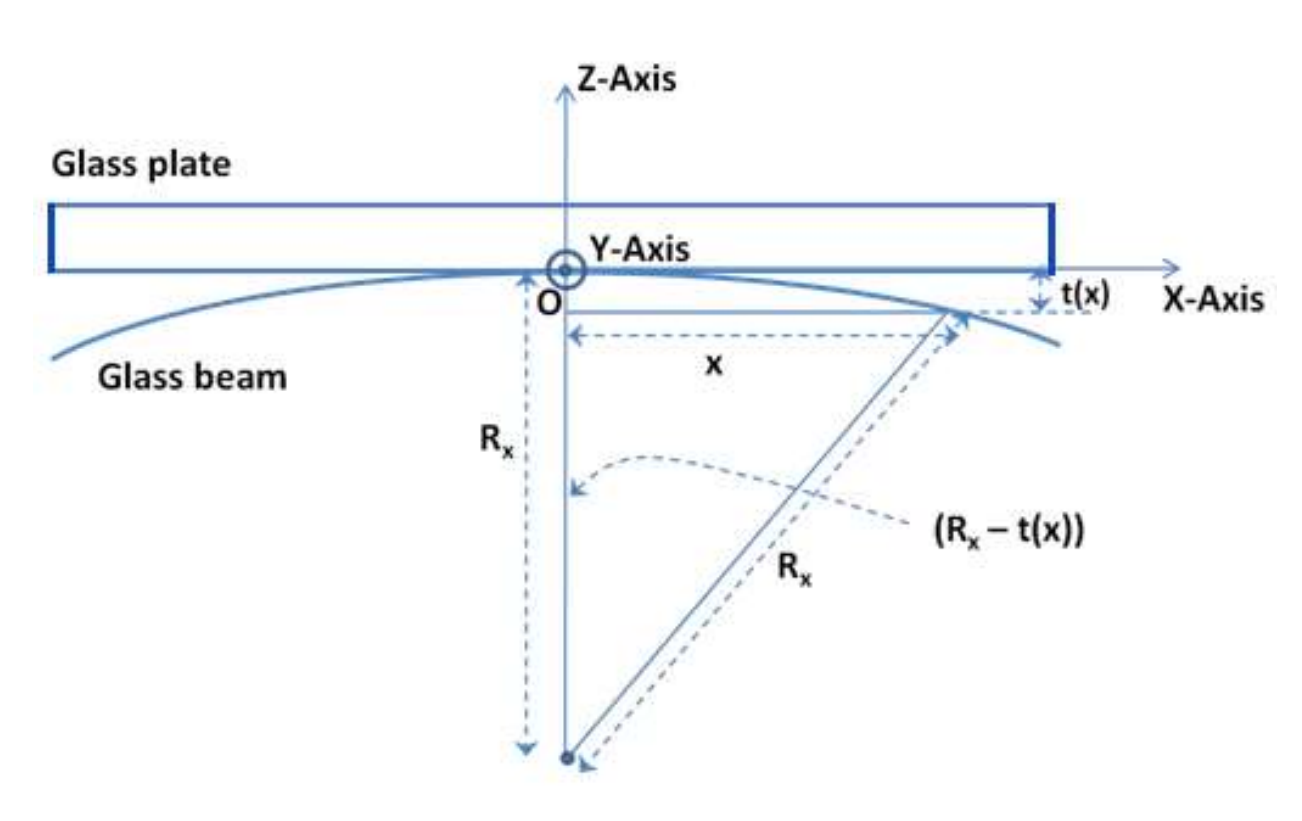
\includegraphics[width=0.7\columnwidth]{images/f1.png}
    \caption{Schematic of the experimental setup (Quincke's tube)}
    \label{fig:1}
\end{figure}

Suppose that, when the field is turned on, the meniscus in the narrow tube rises by an amount $h$, relative to its zero-field position. A volume $\pi r^2h$ of air in the narrow tube is, therefore, replaced by liquid. Hence, the magnetic potential energy of this volume of space increases by

\begin{equation}
    \Delta U = \frac{1}{2}(\mu-\mu_\text{air})H^2\cdot\pi r^2h
\end{equation}

Which is equal to the work done by the magnetic force $\vect{F}_m$ in raising the liquid by an amount $h$.

\begin{equation}
    F_m = \frac{\Delta U}{h} = \frac{1}{2}(\mu-\mu_\text{air})H^2\pi r^2
\end{equation}

When the liquid in one arm of the tube rises by $h$, it falls on the other arm by $h$. It continues to rise till the upward magnetic force is balanced by the weight of the head of liquid. The downward gravitational force on the head of liquid, of mass $m$, is given by

\begin{equation}
    F_g = mg = 2\pi r^2 \rho h g
\end{equation}

where $\rho$ is the density of the liquid. There is also a very small additional upwards force on the liquid due to the buoyancy of the air, displaced by the liquid, given by

\begin{equation}
    F_b = 2\pi r^2 \rho_\text{air} h g
\end{equation}

When the forces are balanced, we have $F_m + F_b = F_g $, 

\begin{equation}
    \frac{1}{2}(\mu-\mu_\text{air})H^2\pi r^2 = 2\pi r^2 (\rho - \rho_\text{air}) h g
\end{equation}

Substituting $H$ from Eq.(4) in Eq.(9), we rearrange to get
\begin{equation}
    \chi = \frac{h}{B^2}[4g\mu_o(\rho - \rho_\text{air})] - \chi_\text{air}
\end{equation}

where $\chi$ is the total susceptibility of the solution $\chi = \chi_\text{Fe} + \chi_\text{water}$. From this, we can calculate certain other parameters like,

\begin{itemize}
    \item mass susceptibility, $\chi' = \chi/\rho$
    \item molar susceptibility, $\chi'' = \chi'M$
    \item Curie constant, $C = \chi''T$
    \item Magnetic moment of dipole of the specimen, $\mu=2.8241\sqrt{C}$
\end{itemize}

where $M$ = Molecular Weight, $T$ = Temperature of the specimen.


Everything here assumes that the magnetic field acting on each ion is just the applied field $B$, and field and contributions due to neighboring magnetic ions are neglected. For dilute paramagnetic materials these other contributions are very small and the approximation is valid. This is not so for concentrated magnetic materials and ferromagnets. 



\section{Experimental Setup}
Quincke’s tube is U-shaped glass tube (Fig.1).  One arm of the tube is placed
between the pole-pieces of an electromagnet shown as N-S such that the meniscus of the liquid lies symmetrically between N-S. The length of the limb is sufficient as to keep the other lower extreme end of this limb well outside the field H of the magnet. The rise or fall $h$ is measured by means of a traveling microscope.

\begin{figure}[H]
    \centering
    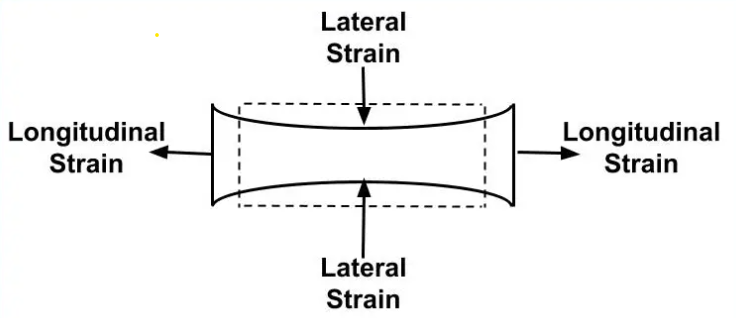
\includegraphics[width=0.8\columnwidth]{images/f2.png}
    \caption{Experimental setup}
    \label{fig:enter-label}
\end{figure}

\subsection{Apparatus}
\begin{enumerate}
    \item Adjustable electromagnet with pole pieces
    \item Constant power supply (0-16 V, 5A DC)
    \item Digital Gauss meter
    \item Hall probe for magnetic strength measurement
    \item Travelling Microscope
    \item Quincke’s tube (an U tube)
    \item Measuring cylinder (100ml), dropper, Wash bottle
    \item Specific gravity bottle
    \item FeCl$_3$ for making solutions
    \item Electronic balance
    \item Connecting cords 

\end{enumerate}
    \section{Observations and Calculations}

    \subsection{Observational Data}
    \begin{itemize}
        \item Least count of the micrometer = 0.01mm
        \item Breadth of the glass slab ($b$) = 49.4mm
        \item Depth of the glass slab ($d$) = 2.07mm
        \item Distance from the knife-edge to the load ($l$) = 115mm
        \item Wavelength of the monochromatic light used ($\lambda$) = 589.3nm
    \end{itemize}
    
    \subsubsection{For $\text{m}_1$ = 200g}
        \begin{table}[H]
    \centering
    \begin{tabular}{|c|c|c|c|c|c|}
        \hline
        Fringe    & Fringes on     & Fringes on       & $\text{D}_x$        & $\rho_x$   & $\text{R}_x$    \\ 
        Order     & the left (mm)  & the right (mm)   & (mm)       & ($\text{mm}^2$)   & (mm)   \\ \hline
        1 &  9.24 & 5.40 &  3.84 &     &     \\
         2 & 10.38 & 3.89 &  6.49 &  6.84 & 11.62 \\
         3 & 11.18 & 3.02 &  8.16 & 12.96 & 11.00  \\
         4 & 12.41 & 2.23 & 10.18 & 22.22 & 12.58 \\
         5 & 13.05 & 1.48 & 11.57 & 29.78 & 12.64 \\
         6 & 13.55 & 0.82 & 12.73 & 36.83 & 12.50 \\
         7 & 14.10 & 0.18 & 13.92 & 44.76 & 12.66 \\\hline
       \end{tabular}
    \caption{Observed fringe pattern on along the longitudinal direction}
    \label{tab:3}
\end{table}
        \begin{table}[H]
    \centering
    \begin{tabular}{|c|c|c|c|c|c|}
        \hline
        Fringe    & Fringes on     & Fringes on       & $\text{D}_y$        & $\rho_y$   & $\text{R}_y$    \\ 
        Order     & the bottom (mm)  & the top (mm)   & (mm)       & ($\text{mm}^2$)   & (mm)   \\ \hline
        1 & 17.5 & 8.01  &  9.49 &       &     \\
        2 & 20.02 & 6.55 & 13.47 &  22.85 & 38.79 \\
        3 & 22.24 & 5.01 & 17.23 &  51.70 & 43.89 \\
        4 & 24.07 & 4.52 & 19.55 &  73.04 & 41.33 \\
        5 & 25.99 & 3.53 & 22.46 & 103.60 & 43.97 \\
        \hline
       \end{tabular}
    \caption{Observed fringe pattern on along the transverse direction}
    \label{tab:4}
\end{table}

        
    \subsubsection{For $\text{m}_2$ = 250g}
        \begin{table}[H]
    \centering
    \begin{tabular}{|c|c|}
    \hline
     I(A)& B (Gauss) \\ \hline
     0.0 &    0 \\
     0.2 &  188 \\
     0.4 &  389 \\
     0.6 &  568 \\
     0.8 &  780 \\
     1.0 &  988 \\
     1.2 & 1170 \\
     1.4 & 1350 \\
     1.6 & 1580 \\
     1.8 & 1770 \\
     2.0 & 1980 \\
     2.2 & 2170 \\
     2.4 & 2360 \\
     2.6 & 2540 \\
     2.8 & 2740 \\
     3.0 & 2940 \\
     3.2 & 3130 \\
     3.4 & 3340 \\
     3.5 & 3420 \\
     3.6 & 3500 \\
     3.7 & 3600 \\
     3.8 & 3690 \\
     3.9 & 3790 \\
     4.0 & 3870 \\
    \hline
    \end{tabular}
    \caption{Data for calibration}
    \label{tab:1}
\end{table}
        \begin{table}[H]
    \centering
    \begin{tabular}{|c|c|c|c|c|c|}
        \hline
        Fringe    & Fringes on     & Fringes on       & $\text{D}_y$        & $\rho_y$   & $\text{R}_y$    \\ 
        Order     & the bottom (mm)  & the top (mm)   & (mm)       & ($\text{mm}^2$)   & (mm)   \\ \hline
        1 & 15.21 & 9.6  &  5.61 &     &     \\
        2 & 18.00 & 6.97 & 11.03 &  22.55 & 38.28 \\
        3 & 19.99 & 5.66 & 14.33 &  43.47 & 36.90 \\
        4 & 21.66 & 4.72 & 16.94 &  63.87 & 36.15 \\
        5 & 23.36 & 3.84 & 19.52 &  87.39 & 37.09 \\
        6 & 25.62 & 3.40 & 22.22 & 115.56 & 39.24 \\
        \hline
       \end{tabular}
    \caption{Observed fringe pattern on along the transverse direction}
    \label{tab:2}
\end{table}

    \subsubsection{For $\text{m}_3$ = 300g}
        \begin{table}[H]
    \centering
    \begin{tabular}{|c|c|c|c|c|c|}
        \hline
        Fringe    & Fringes on     & Fringes on       & $\text{D}_x$        & $\rho_x$   & $\text{R}_x$    \\ 
        Order     & the left (mm)  & the right (mm)   & (mm)       & ($\text{mm}^2$)   & (mm)   \\ \hline
        1 & 13.03 & 9.94 &  3.09 &      &     \\
         2 & 14.24 & 9.04 &  5.20  &  4.37 & 7.42 \\
         3 & 15.00 & 8.37 &  6.63 &  8.60 & 7.30 \\
         4 & 16.17 & 7.82 &  8.35 & 15.04 & 8.51 \\
         5 & 16.69 & 7.38 &  9.31 & 19.28 & 8.18 \\
         6 & 17.10 & 6.91 & 10.19 & 23.57 & 8.00  \\
         7 & 17.56 & 6.51 & 11.05 & 28.14 & 7.96 \\
         8 & 17.98 & 6.12 & 11.86 & 32.78 & 7.95 \\\hline
       \end{tabular}
    \caption{Observed fringe pattern on along the longitudinal direction}
    \label{tab:1}
\end{table}
        \begin{table}[H]
    \centering
    \begin{tabular}{|c|c|c|c|c|c|}
        \hline
        Fringe    & Fringes on     & Fringes on       & $\text{D}_y$        & $\rho_y$   & $\text{R}_y$    \\ 
        Order     & the bottom (mm)  & the top (mm)   & (mm)       & ($\text{mm}^2$)   & (mm)   \\ \hline
        1 & 15.48 & 10.64 &  4.84 &       &      \\
         2 & 17.95 &  7.84 & 10.11 &  19.70 & 33.44 \\
         3 & 19.76 &  5.68 & 14.08 &  43.71 & 37.10 \\
         4 & 21.29 &  4.26 & 17.03 &  66.65 & 37.72 \\
         5 & 21.85 &  3.07 & 18.78 &  82.32 & 34.94 \\
         6 & 22.69 &  1.99 & 20.70 & 101.27 & 34.39 \\
         7 & 23.47 &  0.91 & 22.56 & 121.38 & 34.35 \\
        \hline
       \end{tabular}
    \caption{Observed fringe pattern on along the transverse direction}
    \label{tab:2}
\end{table}

    \subsection{Calculations}
    \subsubsection{Calculation of Young's Modulus (Y)}

     We can rearrange equation (14) to form 

    \begin{equation}
        \left(\frac{1}{\rho_{x}^1(s)}-\frac{1}{\rho_{x}^2(s)}\right)^{-1} = \left(\frac{Ybd^3\lambda}{12gl(m_1-m_2)}\right)s
    \end{equation}

    which is of form $y=mx+c$, where $m=$ slope and $c=$ y-intercept of a straight line. Thus we can plot the LHS of this eqn. vs $s$ to find out $Y$ using,

    \begin{equation}
        Y = \frac{12gl(m_1-m_2)}{bd^3\lambda}\cdot m
    \end{equation}
    
    \begin{figure}[H]
        \centering
        \label{graph:1}
        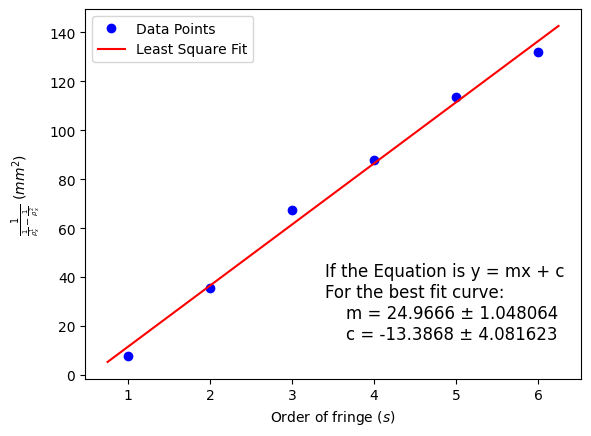
\includegraphics[width=0.8\columnwidth]{images/1.png}
        \caption{$(\frac{1}{\rho_{x}^1}-\frac{1}{\rho_{x}^2})^{-1}$ vs Order of fringe $(s)$}
    \end{figure}

    \begin{figure}[H]
        \centering
        \label{graph:2}
        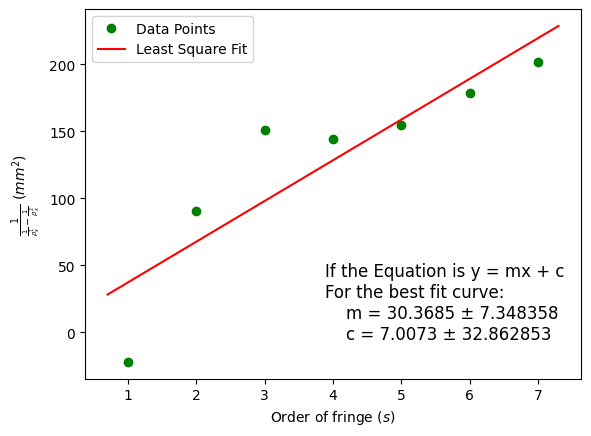
\includegraphics[width=0.8\columnwidth]{images/2.png}
        \caption{$(\frac{1}{\rho_{x}^2}-\frac{1}{\rho_{x}^3})^{-1}$ vs Order of fringe $(s)$}
    \end{figure}

    \begin{figure}[H]
        \centering
        \label{graph:3}
        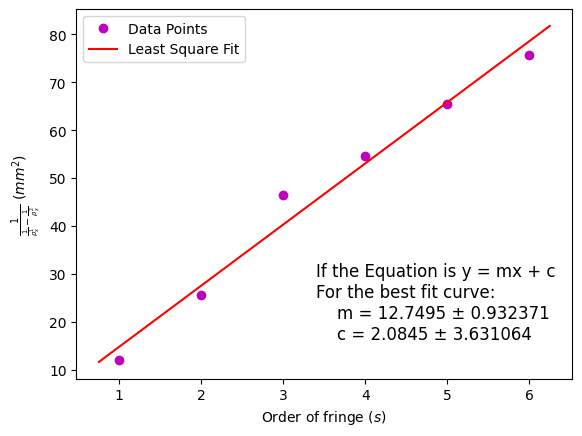
\includegraphics[width=0.8\columnwidth]{images/3.png}
        \caption{$(\frac{1}{\rho_{x}^1}-\frac{1}{\rho_{x}^3})^{-1}$ vs Order of fringe $(s)$}
    \end{figure}

    Using eq. (18),
   \begin{itemize}
       \item For $m_1$ and $m_2$, $Y_{12}$ = 66.80 GPa
       \item For $m_2$ and $m_3$, $Y_{23}$ = 75.34 GPa
       \item For $m_1$ and $m_3$, $Y_{13}$ = 66.88 GPa
   \end{itemize}

   Thus, average value of Y = 69.67 GPa

   \subsubsection{Calculation of Poisson's Ratio ($\sigma$)}

     We can rearrange equation (16) to form 
     \begin{equation}
         \rho_x(s) = \sigma \rho_y(s)
     \end{equation}

      which is of form $y=mx+c$, where $m=$slope and $c=$ y-intercept of a straight line. Thus we can plot this $rho_x(s)$ vs $\rho_y(s)$ to find out $\sigma$ which is equal to the slope ($m$).

      \begin{figure}[H]
        \centering
        \label{graph:4}
        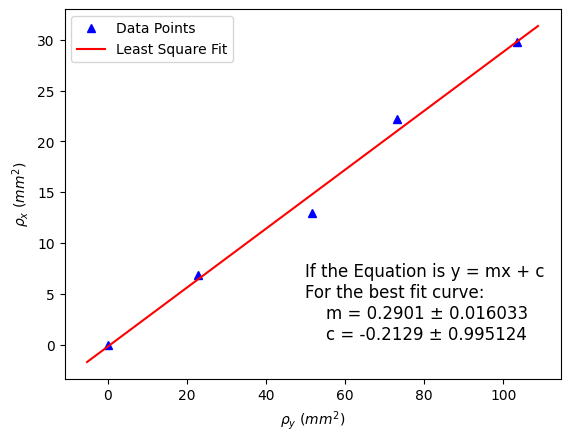
\includegraphics[width=0.8\columnwidth]{images/4.png}
        \caption{Si diode in forward bias}
    \end{figure}

    \begin{figure}[H]
        \centering
        \label{graph:5}
        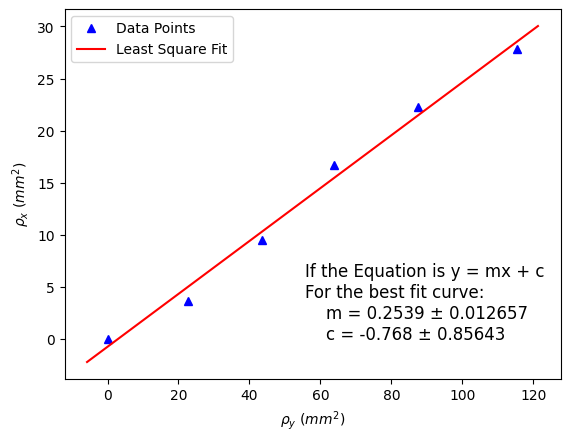
\includegraphics[width=0.8\columnwidth]{images/5.png}
        \caption{$\rho_x$ vs $\rho_y$ for m = 250g}
    \end{figure}

    \begin{figure}[H]
        \centering
        \label{graph:6}
        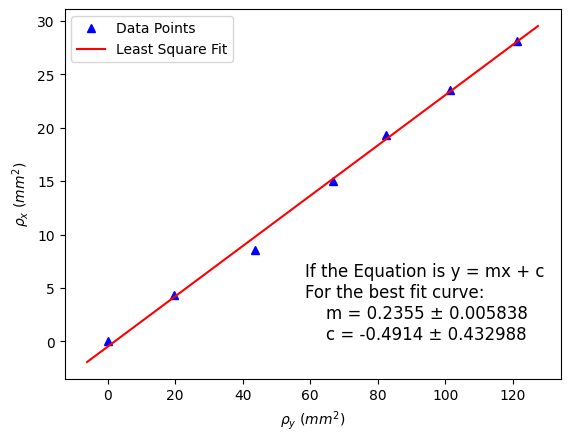
\includegraphics[width=0.8\columnwidth]{images/6.png}
        \caption{$\rho_x$ vs $\rho_y$ for m = 300g}
    \end{figure}

    Thus, the average value of $\sigma$ is observed to be 0.261.
    \section{Error Analysis}
\begin{enumerate}
    \item Error in $\rho$:
        \begin{align*}
            \Delta \rho = \sqrt{\left(\frac{\partial \rho}{\partial w_1}\Delta w_1\right)^2 + \left(\frac{\partial \rho}{\partial w_2}\Delta w_2\right)^2 + \left(\frac{\partial \rho}{\partial w_3}\Delta w_3\right)^2}\\          
            \frac{\Delta \rho}{\rho} = \sqrt{\frac{(\Delta w_1)^2(w_3-w_2)^2}{(w_2-w_1)^2(w_3-w_1)^2} + \left(\frac{\Delta w_2}{w_2-w_1}\right)^2 + \left(\frac{\Delta w_3}{w_3-w_1}\right)^2}
        \end{align*}
        \begin{align*}
            \therefore \Delta \rho = 6.7\,kg/m^3
        \end{align*}
    \item Error in $\chi_\text{Fe}$:
        \begin{align*}
            \frac{\Delta \chi_\text{Fe}}{\chi_\text{Fe}} &= \sqrt{\left(\frac{\Delta \text{slope}}{\text{slope}}\right)^2 + \left(\frac{\Delta \rho}{\rho - \rho_\text{air}}\right)^2}\\
            \Delta \chi_\text{Fe} &= 0.03 \times 10^{-5}
        \end{align*}
    \item Error in $\chi'_\text{Fe}$:
        \begin{align*}
            \frac{\Delta \chi'_\text{Fe}}{\chi'_\text{Fe}} &= \sqrt{\left(\frac{\Delta \chi_\text{Fe}}{\chi_\text{Fe}}\right)^2 + \left(\frac{\Delta \rho}{\rho}\right)^2}\\
            \Delta \chi'_\text{Fe} &= 0.03 \times 10^{-8}\,m^3/kg 
        \end{align*}
    \item Error in $\chi''_\text{Fe}$:
        \begin{align*}
            \frac{\Delta \chi''_\text{Fe}}{\chi''_\text{Fe}} &= \sqrt{\left(\frac{\Delta \chi'_\text{Fe}}{\chi'_\text{Fe}}\right)^2}\\
            \Delta \chi''_\text{Fe} &= 0.005 \times 10^{-8}\,m^3/mol 
        \end{align*}
    \item Error in $C$:
        \begin{align*}
            \frac{\Delta C}{C} &= \sqrt{\left(\frac{\Delta \chi''_\text{Fe}}{\chi''_\text{Fe}}\right)^2 + \left(\frac{\Delta T}{T}\right)^2}\\
            \Delta C &= 0.02 \times 10^{-6}\,m^3\,K/mol
        \end{align*}
    \item Error in $\mu$:
        \begin{align*}
            \frac{\Delta \mu}{\mu} &= \sqrt{\left(\frac{\Delta C}{2C}\right)^2}\\
            \Delta \mu &= 0.02 \times 10^{-3}\,A/m^2 
        \end{align*}
\end{enumerate}
    \section{Results}
From the experiment, I have measured the value of Young's modulus (Y) and Poisson's ratio ($\sigma$) of the given glass slab to be,
\begin{align*}
    \text{Y} &= 69.67 \pm 6.03 \text{ GPa} \\
    \sigma   &= 0.261 \pm 0.007
\end{align*}\\[0.5pt]



    \section{Conclusion}
Our measured values of Young's modulus and Poisson's ratio is within the the literature values of Y = 50 to 90 GPa and $\sigma$ = 0.2 to 0.7 respectively.

Glass is a brittle material and thus shows very little strain subject to a considerable amount of stress upto the elastic limit. Thus, the high value of Young's modulus observed is justified.

Using this experiment, we can determine the refractive index of an unknown liquid by substituting it with the air-film.

\section{Precautions \& Sources of Error}
\begin{enumerate}
    \item The beam should be placed on the knife–edges symmetrically.
    \item All the glass plates must be plane (optically) and clean.
    \item The travelling microscope must be handled carefully in order to avoid backlash error.
\end{enumerate}
    

    \bibliographystyle{apalike}
    \bibliography{ref.bib}
    \nocite{*}
\end{document}